\documentclass[tikz,border=2pt]{standalone}
\usepackage{amsmath}
\usetikzlibrary{arrows.meta}
\begin{document}
% Two stages for a package: install.packages("readr") once per computer (archive -> disk),
% library(readr) in every session (disk -> session), after which read_csv() can be called.
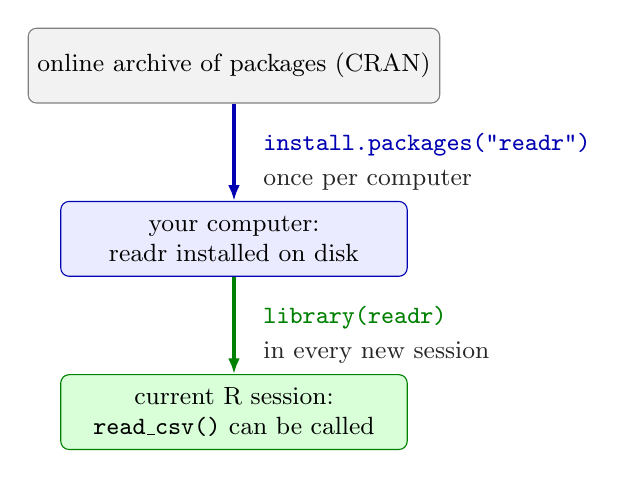
\begin{tikzpicture}[font=\small, >={Latex[length=2mm]},
  box/.style={draw, rounded corners=3pt, minimum width=4.4cm, minimum height=0.95cm, align=center},
  cmd/.style={anchor=west, font=\small\ttfamily}]
  \node[box, draw=gray, fill=gray!10] (a) at (0,0) {online archive of packages (CRAN)};
  \node[box, draw=blue!70!black, fill=blue!8] (b) at (0,-2.2) {your computer:\\ readr installed on disk};
  \node[box, draw=green!50!black, fill=green!15] (c) at (0,-4.4) {current R session:\\ \texttt{read\_csv()} can be called};
  \draw[->, very thick, blue!70!black] (a) -- (b);
  \draw[->, very thick, green!50!black] (b) -- (c);
  \node[cmd, blue!70!black] at (0.25,-1.0) {install.packages("readr")};
  \node[anchor=west, gray!30!black] at (0.25,-1.45) {once per computer};
  \node[cmd, green!50!black] at (0.25,-3.2) {library(readr)};
  \node[anchor=west, gray!30!black] at (0.25,-3.65) {in every new session};
\end{tikzpicture}
\end{document}
